\documentclass[review,10pt]{elsarticle}

\usepackage[utf8]{inputenc}
\usepackage[T1]{fontenc}
\usepackage{amsmath}
\usepackage{amssymb}
\usepackage{booktabs}
\usepackage{graphicx}
\usepackage{algorithm}
\usepackage{algorithmic}
\usepackage{xcolor}
\usepackage{multirow}
\usepackage{hyperref}
\usepackage{float}
\usepackage{dblfloatfix}

\journal{Pattern Recognition}

\begin{document}

\begin{frontmatter}

\title{Test-Time Adaptation for Image Demoir\'{e}ing: An Adapter-Based Framework with Frequency-Aware Self-Supervision}

\author[hnu]{Yu Qiu}
\ead{qiuyu123@hnu.edu.cn}
\address[hnu]{School of Mathematics, Hunan University, Changsha 410082, China}

\begin{abstract}
Moir\'{e} patterns --- frequency aliasing artifacts from camera-screen interference --- remain a persistent challenge in computational photography. While deep learning methods achieve strong results on trained device-screen combinations, their performance degrades when deployed on unseen capture setups, owing to severe domain overfitting. We propose MoTA (Moir\'{e} Test-Time Adaptation), an adapter-based framework that enables pre-trained demoir\'{e}ing backbones to adapt at inference time without paired target-domain data. MoTA inserts a lightweight Fourier Domain Adapter (FDA, $\sim$1\% of backbone parameters) into a frozen backbone, guided by a Moir\'{e}-Aware Self-Supervision (MASS) signal that generates pseudo-clean targets via selective frequency-band attenuation of wavelet mid-frequency subbands. On the LCDMoire in-domain benchmark, FDA-based MoTA with WDNet backbone achieves +2.57 dB PSNR over frozen inference, surpassing a LoRA baseline (rank=4, +1.82 dB) with fewer trainable parameters. This in-domain improvement does not transfer to the cross-domain setting: on TIP2018, MoTA performs below the frozen WDNet baseline (16.00 dB vs.\ 18.91 dB). Through quantitative diagnostics on a preliminary 100-image subset, we identify degraded self-supervision quality as the primary bottleneck --- pseudo-clean targets generated by the source-domain-trained detector achieve lower PSNR than the frozen model output on the target domain (pending full-set verification). A Spatial Gating Adapter (SGA) variant is explored but found to compete with FDA at shared insertion points. These findings establish a baseline for adapter-based test-time adaptation in demoir\'{e}ing and characterize key failure modes under domain shift.
\end{abstract}

\begin{keyword}
image demoir\'{e}ing \sep test-time adaptation \sep self-supervision \sep adapter \sep wavelet transform \sep domain generalization
\end{keyword}

\end{frontmatter}
\section{Introduction}

When a digital camera captures a screen display, the superposition of the camera's color filter array and the screen's pixel grid produces aliasing artifacts known as moir\'{e} patterns --- irregular, colorful fringes that severely degrade image quality. As smartphone photography of screens becomes ubiquitous in daily life --- from photographing documents and QR codes to sharing social media posts --- the demand for robust demoir\'{e}ing continues to grow. Over the past five years, a substantial body of deep learning research has tackled this problem \cite{sun2018moire,zheng2022learning,he2020fhde2net,yu2022towards,guo2025moirenet}, steadily pushing PSNR on standard benchmarks from $\sim$26 dB to over 30 dB on TIP2018.

Despite this progress, a critical vulnerability remains underappreciated: \textbf{domain overfitting}. Existing demoir\'{e}ing models are trained and evaluated on images captured from a fixed set of device-screen combinations, typically one or two smartphone models photographing IPS LCD panels at $1\times$ zoom. When deployed on a different device, panel type, or zoom level, performance degrades sharply --- a 3--5 dB PSNR drop is common \cite{yang2025unidemoire}. This fragility stems from the fundamental nature of moir\'{e}: unlike Gaussian noise or uniform blur, moir\'{e} patterns are determined by the specific physical parameters of the capture pipeline (sensor pixel pitch, screen dot pitch, shooting distance, lens characteristics), and each unseen combination produces a qualitatively different aliasing pattern \cite{patel2016survey}. Data-centric approaches like UniDemoir\'{e} \cite{yang2025unidemoire} attempt to cover more of this diversity by collecting larger moir\'{e} pattern libraries and synthesizing augmented training images, but the combinatorial space of possible capture configurations is ultimately unbounded.

Test-time adaptation (TTA) offers an orthogonal approach to domain overfitting: rather than trying to anticipate every possible domain during training, TTA methods adjust model parameters at inference time using only the input image itself. Foundational TTA methods include self-supervised test-time training \cite{sun2020ttt} and entropy minimization \cite{wang2021tent}, with subsequent work addressing stability \cite{niu2023towards} and augmentation \cite{zhang2022memo}. In image restoration, TTA has been applied to all-in-one restoration via degradation-consistent adaptation \cite{tang2026degradation}, open-set degradation handling \cite{gou2024testtime}, and preference optimization \cite{li2026testtime}. Unlike domain adaptation which aligns distributions during training~\cite{ganin2016domain,kouw2019review}, TTA performs alignment at inference with no source data access. This paradigm has shown promise for handling unseen degradations in denoising \cite{mansour2024tttmim}, super-resolution \cite{deng2023efficient}, and all-in-one restoration \cite{tang2026degradation}. Existing TTA methods, however, are designed for generic degradations and lack mechanisms specific to the frequency-domain nature of moir\'{e}. Most also require full model updates --- risking catastrophic forgetting on single-image adaptation --- or are architecturally constrained, precluding use with arbitrary backbone networks. Moir\'{e}XNet \cite{li2025moirexnet} is the only prior work combining test-time training with demoir\'{e}ing, but its TTT mechanism is embedded within linear attention layers, tying adaptation to a single architecture.

We propose \textbf{MoTA (Moir\'{e} Test-Time Adaptation)}, an adapter-based framework that explores the potential and limits of test-time adaptation for cross-domain image demoir\'{e}ing. MoTA inserts a lightweight Fourier Domain Adapter (FDA) module into a frozen pre-trained demoir\'{e}ing backbone. At inference, only the FDA is updated ($<$2\% of total parameters), guided by a \textbf{Moir\'{e}-Aware Self-Supervision (MASS)} signal. MASS exploits a key property of moir\'{e}: the aliasing energy concentrates in mid-frequency subbands (LH and HL of a wavelet decomposition), while low-frequency content and high-frequency texture occupy separate bands. By detecting moir\'{e}-affected frequency regions and selectively attenuating them, MASS generates a pseudo-clean target that provides effective supervision for adapter optimization --- no paired target-domain data, specialized hardware, or multi-frame capture is required.

This work makes three contributions:
\begin{itemize}\raggedright
    \item \textbf{MoTA}, an adapter-based test-time adaptation framework for image demoir\'{e}ing. A lightweight Fourier Domain Adapter (FDA, ${<}2$\% backbone parameters) is inserted into a frozen pre-trained demoir\'{e}ing backbone and updated at inference time, with full TTA evaluation on WDNet and frozen baseline comparison on DDA/MBCNN.
    \item \textbf{MASS (Moir\'{e}-Aware Self-Supervision)}, a frequency-selective self-supervision signal that leverages the band-limited nature of moir\'{e} energy in wavelet subbands to generate pseudo-clean targets from a single input image.
    \item An \textbf{empirical characterization of adapter-based TTA under domain shift}, documenting the gap between in-domain and cross-domain performance and identifying self-supervision quality degradation as the primary failure mode.
\end{itemize}

\section{Related Work}

\subsection{Image Demoir\'{e}ing}

Image demoir\'{e}ing aims to remove moir\'{e} patterns --- frequency aliasing artifacts caused by the interference between camera sensor grids and screen pixel arrays. Early deep learning approaches tackled this with multi-scale convolutional architectures. Sun et al. \cite{sun2018moire} pioneered the field with a multi-resolution CNN trained on the TIP2018 dataset. Recognizing that moir\'{e} is fundamentally a frequency-domain phenomenon \cite{liu2025fourier}, subsequent methods shifted toward explicit frequency decomposition. Zheng et al. \cite{zheng2022learning} proposed learnable DCT-based bandpass filters (MBCNN) to extract frequency priors, winning the AIM 2019 demoir\'{e}ing challenge. Liu et al. \cite{liu2020wavelet} introduced wavelet-domain dual-branch processing (WDNet) to separate moir\'{e} frequencies from image content. He et al. \cite{he2020fhde2net} designed a frequency disentangling network (FHDe2Net) with a dedicated DCT branch for full-HD images.

More recently, the trend has moved toward deeper frequency-spatial fusion. Moir\'{e}Net \cite{guo2025moirenet} achieved state-of-the-art results with a compact dual-domain CNN (5.5M parameters) featuring directional frequency-spatial encoding, while WDNet \cite{liu2020wavelet} processes images in the wavelet transform domain with dual-branch subband processing. A common limitation of these methods is their reliance on \textbf{fixed} frequency decomposition strategies (DWT, DCT, or learned but static filters) that cannot adapt to the diverse frequency characteristics of moir\'{e} patterns across different capture devices and screen types. This rigidity fundamentally limits their cross-domain generalization.

Concurrently, CLEAR \cite{zhu2026clear} (CVPR 2026) addresses the joint removal of flicker-banding and moir\'{e} artifacts in screen-captured images, introducing a new dataset and frequency-domain decomposition approach --- complementary to our TTA-based domain adaptation focus.

\subsection{High-Resolution and Efficient Demoir\'{e}ing}

As smartphone cameras routinely capture 4K+ images, efficient high-resolution demoir\'{e}ing has gained attention. Yu et al. \cite{yu2022towards} proposed ESDNet with scale-aware modules and the UHDM 4K dataset. Xiao et al. \cite{xiao2024pbic} exploited the green channel's relative immunity to moir\'{e} for patch-level detail transfer (P-BiC). MFFNet \cite{chen2025mffnet} introduced the first joint demoir\'{e}ing and super-resolution framework. DDA \cite{zhang2023dda} targeted real-time mobile deployment. These methods are trained and evaluated within a single data distribution and offer no mechanism to adapt when deployed on unseen capture setups. General image restoration has also advanced with Transformer-based architectures such as SwinIR~\cite{liang2021swinir} and Restormer~\cite{zamir2022restormer}, though these are likewise trained for fixed degradation models without test-time adaptation capability.

\subsection{RAW-Domain and Multi-Domain Demoir\'{e}ing}

Since moir\'{e} originates in the camera's RAW capture before ISP processing, several recent works exploit RAW-domain information. Xu et al. \cite{xu2024image} proposed RRID (ECCV 2024), jointly utilizing RAW and sRGB data through a Spatial-Channel Demoir\'{e}ing Module. Li et al. \cite{li2025moirexnet} extended RAW-domain processing to multi-frame inputs with Moir\'{e}XNet, which incorporates linear attention Test-Time Training (TTT) layers that update during inference and a Truncated Flow Matching Prior for detail recovery. Moir\'{e}XNet represents the only prior work combining test-time training with demoir\'{e}ing, but differs from MoTA in four key aspects: (i) TTT scope --- Moir\'{e}XNet updates only attention weights within linear attention layers, while MoTA updates dedicated adapter parameters (FDA) inserted at intermediate layers of the backbone via forward hooks; (ii) input requirements --- Moir\'{e}XNet requires multi-frame RAW bursts, while MoTA operates on single sRGB images; (iii) computational cost --- Moir\'{e}XNet's TTT updates $\sim$30\% of parameters per step (estimated from architecture; not reported in the original paper) vs.\ MoTA's $<$2\%; (iv) architecture dependence --- Moir\'{e}XNet's TTT is bound to its linear attention design, whereas MoTA inserts lightweight adapters via forward hooks, a design that is architecturally separable from the backbone. DemMamba \cite{xu2024demmamba} applied state space models (Mamba) for alignment-free RAW video demoir\'{e}ing. Despite the demonstrated value of RAW information, these methods either require RAW capture at inference time --- unavailable on most consumer devices --- or, as with Moir\'{e}XNet, bind the TTT mechanism to specific architectural components, preventing application to other backbone architectures.

\subsection{Video, Data-Centric, and Universal Demoir\'{e}ing}

Video demoir\'{e}ing adds temporal consistency challenges addressed by DTNet \cite{xu2024direction} (AAAI 2024, direction-aware DCT detection) and FPANet \cite{oh2025fpanet} (frequency-domain frame-level post-alignment). For data generation and unpaired learning, UniDemoir\'{e} \cite{yang2025unidemoire} (AAAI 2025) collected 150K real moir\'{e} patterns and used diffusion models for synthesis. UnDeM \cite{zhong2024undem} learned from unpaired data, and SIDME \cite{wang2025sidme} explored self-supervised masked reconstruction. These data-centric approaches broaden training distributions but remain limited by data coverage --- truly unseen domains still cause degradation. In Pattern Recognition, frequency-domain processing has been applied to restoration: Gao et al.~\cite{gao2025fdt} proposed frequency-gated networks, Wu et al.~\cite{wu2025freprompter} introduced frequency self-prompting, and Song et al.~\cite{song2025fddm} developed frequency-domain diffusion for underwater enhancement. These do not address moir\'{e}-specific domain overfitting or test-time adaptation.

\subsection{Test-Time Adaptation for Image Restoration}

Test-time adaptation (TTA) has emerged as a promising paradigm for handling distribution shifts in image restoration without requiring target-domain training data. Tang et al. \cite{tang2026degradation} proposed DCTTA (CVPR 2026), using a diffusion-based re-degradation generator to create pseudo training pairs and selective parameter updates for all-in-one restoration. Gou et al. \cite{gou2024testtime} introduced TAO (ICML 2024 Spotlight), adapting a degradation-agnostic diffusion model to unknown degradations at test time. TTT-MIM \cite{mansour2024tttmim} leveraged masked image modeling as a self-supervised proxy task for denoising distribution shifts. TTPO \cite{li2026testtime} borrowed preference optimization from LLM alignment for test-time refinement. Deng et al. \cite{deng2023efficient} tackled blind super-resolution with second-order degradation modeling and feature-level reconstruction.

Existing TTA methods for image restoration share two limitations in the context of demoir\'{e}ing. They are designed for generic degradations (noise, blur, rain) and lack moir\'{e}-specific adaptation signals --- moir\'{e} patterns differ fundamentally from these degradations in being frequency-aliasing artifacts rather than additive or convolutional corruptions. They also typically require full model updates or architecture-specific modifications, lacking an adapter-based mechanism that can be plugged into arbitrary pre-trained demoir\'{e}ing backbones.

\subsection{Parameter-Efficient Adaptation}

Concurrently, parameter-efficient fine-tuning (PEFT) techniques have been adapted from NLP \cite{houlsby2019adapter} to image restoration. FraIR \cite{korkmaz2026frair} introduced Fourier-domain low-rank adapters with $<$0.5\% trainable parameters. BIR-Adapter \cite{eteke2025biradapter} leveraged frozen diffusion model features through lightweight attention adapters. Edit2Restore \cite{yilmaz2026edit2restore} applied LoRA to the FLUX.1 (12B) model for few-shot restoration. DDOM \cite{wu2026ddom} proposed degradation-oriented adapters (0.36\%--0.63\% parameters) for universal restoration. In parallel, visual prompt tuning \cite{jia2022vpt} and convolutional prompts \cite{chen2023convpass} offer alternative lightweight adaptation paradigms by learning input-space perturbations rather than internal feature modulations. These works demonstrate that lightweight adapters can effectively transfer knowledge to new tasks, but none explore the combination of adapter-based PEFT with test-time adaptation for cross-domain generalization --- a gap our work directly addresses.

Demoir\'{e}ing methods suffer from severe domain overfitting; TTA methods lack moir\'{e}-specific designs and plug-in adapters; and PEFT approaches have not been applied to cross-domain demoir\'{e}ing. \textbf{MoTA (Moir\'{e} Test-Time Adaptation)} bridges these gaps: a test-time adaptation framework with a Moir\'{e}-Aware Self-Supervision (MASS) signal and lightweight adapters that enable pre-trained backbones to adapt at inference time without paired target-domain data.


\section{Method}

\subsection{Overview}

MoTA is an adapter-based test-time adaptation framework for image demoir\'{e}ing. Given a pre-trained demoir\'{e}ing model $f_\theta$ and a test image from an unseen target domain, MoTA adapts the model at inference time without paired data or multi-frame capture from that domain.

The framework comprises three components. First, the \textbf{Moir\'{e}-Aware Self-Supervision (MASS)} module decomposes $I$ into frequency subbands via discrete wavelet transform, detects moir\'{e}-dominant frequency regions, and generates a pseudo-clean target $\tilde{I}$ through selective band attenuation. Second, a \textbf{Fourier Domain Adapter (FDA)} is inserted into the frozen backbone $f_\theta$ to provide a low-dimensional adaptation interface; a Spatial Gating Adapter (SGA) is also explored but found to compete with FDA at shared insertion points (Section~\ref{sec:ablation}). Third, a \textbf{test-time optimization} loop minimizes the discrepancy between the backbone output $\hat{I} = f_{\theta,\phi}(I)$ and $\tilde{I}$ with respect to adapter parameters $\phi$ only; the backbone $\theta$ remains frozen throughout. After $T$ adaptation steps (typical $T=15$), the adapted model produces the final demoir\'{e}d output.

\begin{figure}[tb]
\centering
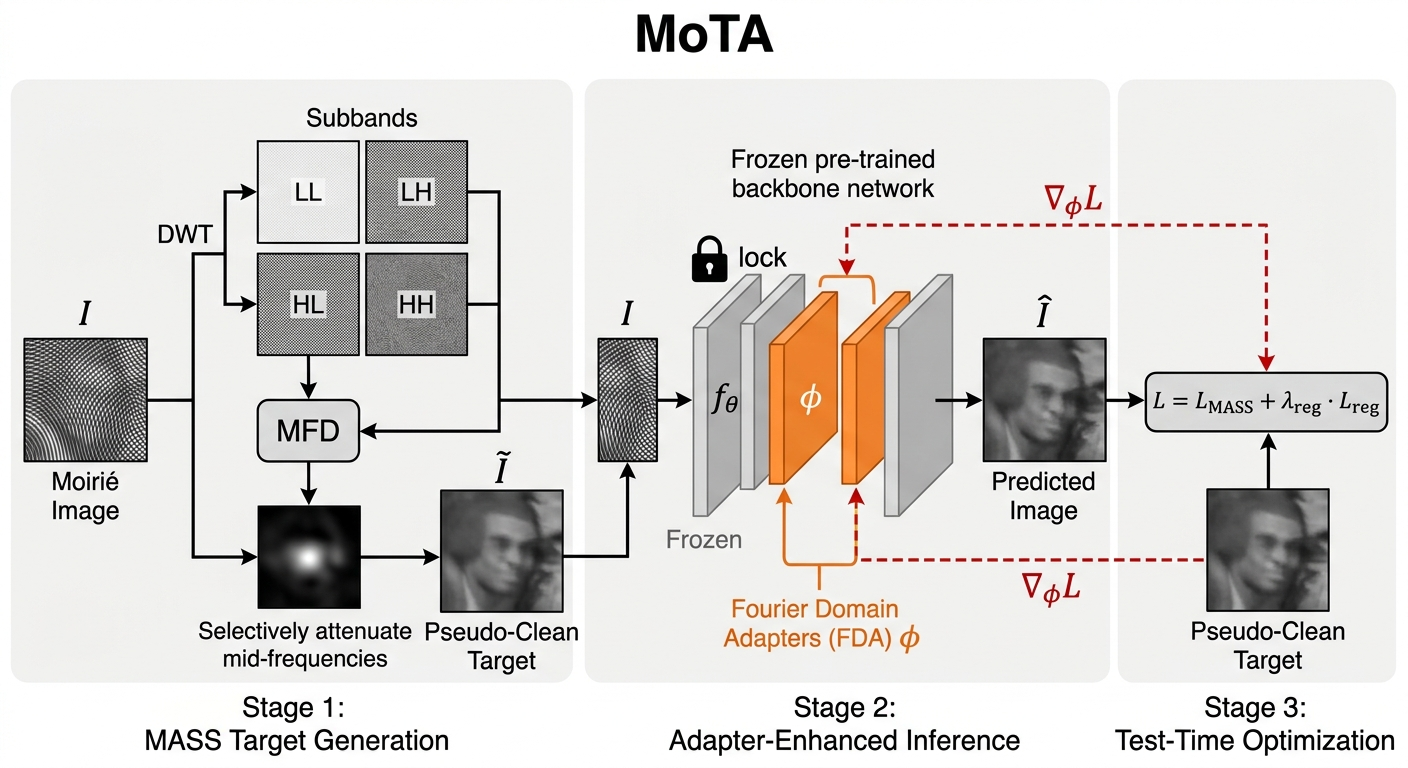
\includegraphics[width=0.95\linewidth]{figures/fig1_framework.jpg}
\caption{MoTA framework overview. Left: Input moir\'{e} image $I$. Middle-top: MASS module generates pseudo-clean target via frequency decomposition and moir\'{e} detection. Middle-bottom: Frozen pre-trained backbone with inserted MoTA Adapter (FDA; an SGA variant is explored in Section~\ref{sec:ablation} but found to compete with FDA). Right: Output $\hat{I}$. A red dashed arrow indicates gradient flow updating only adapter parameters $\phi$ via $\mathcal{L}_{MASS}$. Three colored boxes group the three stages.}
\label{fig:framework}
\end{figure}

\subsection{Preliminaries and Problem Formulation}

\textbf{Image Demoir\'{e}ing.} Let $I_m \in \mathbb{R}^{H \times W \times 3}$ be a moir\'{e}-affected sRGB image and $I_c \in \mathbb{R}^{H \times W \times 3}$ its clean counterpart. A demoir\'{e}ing model $f_\theta: \mathbb{R}^{H \times W \times 3} \to \mathbb{R}^{H \times W \times 3}$ parameterized by $\theta$ is trained to minimize $\mathbb{E}_{(I_m, I_c) \sim \mathcal{D}_S}[\mathcal{L}(f_\theta(I_m), I_c)]$ on a source domain $\mathcal{D}_S$.

\textbf{Domain Shift in Demoir\'{e}ing.} In practice, the test distribution $\mathcal{D}_T$ differs from $\mathcal{D}_S$ because moir\'{e} patterns are determined by capture-specific parameters --- camera sensor, lens, screen type, pixel pitch, shooting distance --- each of which can vary independently. The resulting domain gap causes $f_\theta$ to perform suboptimally on $\mathcal{D}_T$. Our goal is to adapt $\theta$ at test time using only $I_m \sim \mathcal{D}_T$, without access to $I_c$, additional capture hardware, or target-domain training data.

\textbf{Test-Time Adaptation.} We freeze $\theta$ and introduce lightweight adapter parameters $\phi$ (where $|\phi| \ll |\theta|$), yielding an augmented model $f_{\theta,\phi}$. At test time, we optimize $\phi$ on each input $I_m$ via a self-supervised loss $\mathcal{L}_{self}$ that requires no ground truth. After adaptation, the output is $\hat{I} = f_{\theta,\phi_T}(I_m)$.

\textbf{Wavelet Decomposition.} We use the 2D Discrete Wavelet Transform (DWT) with Haar wavelets to decompose images into four subbands: $LL$ (low-frequency approximation), $LH$ (horizontal detail), $HL$ (vertical detail), and $HH$ (diagonal detail). Moir\'{e} energy concentrates in $LH$ and $HL$, a property central to MASS.

\subsection{MoTA Framework Design}

\subsubsection{Architecture Overview}

MoTA's overall pipeline consists of three stages:

\textbf{Stage 1: MASS Signal Generation.} The input image undergoes DWT decomposition. A lightweight Moir\'{e} Frequency Detector (MFD) predicts per-pixel moir\'{e} probability in each frequency subband. Selective attenuation of moir\'{e}-dominant bands produces a pseudo-clean target $\tilde{I}$.

\textbf{Stage 2: Adapter-Enhanced Forward Pass.} The frozen backbone $f_\theta$ processes $I$ with Fourier Domain Adapters (FDA) inserted at intermediate layers (via forward hooks matched to Conv2d output channels), producing an initial estimate $\hat{I}$. A Spatial Gating Adapter (SGA) variant is also explored but found to compete with FDA at shared insertion points (Section~\ref{sec:ablation}).

\textbf{Stage 3: Test-Time Optimization.} The MASS loss $\mathcal{L}_{MASS} = \|\hat{I} - \tilde{I}\|_1$ and regularization $\mathcal{L}_{reg}$ are minimized with respect to $\phi$ over $T$ steps. Only adapter parameters are updated.

\subsubsection{Moir\'{e} Frequency Detector (MFD)}

\textbf{Input:} Single moir\'{e} image $I \in \mathbb{R}^{H \times W \times 3}$

\textbf{Output:} Subband-wise moir\'{e} probability map $M \in \mathbb{R}^{H \times W \times 3}$ (upsampled to input resolution via bilinear interpolation; later downsampled back to subband resolution within MASS)

First, apply single-level Haar DWT to each channel of $I$:
\begin{equation}
\{LL, LH, HL, HH\} = \operatorname{DWT}(I)
\end{equation}

MFD operates on per-channel DWT subbands (3 RGB $\times$ 4 subbands = 12 input channels). For the MASS signal generation (Sec~\ref{sec:mass}), a luminance-channel shortcut is used: DWT is performed on the per-channel mean of RGB, and the resulting correction is broadcast uniformly to all color channels, reducing computation $3\times$ at negligible quality cost.

MFD is a lightweight 4-layer convolutional network that takes the concatenated subbands as input:
\begin{equation}
M = \sigma(\operatorname{MFD}([LL; LH; HL; HH]))
\end{equation}

The three output channels of $M$ correspond to moir\'{e} probability in LH (channel~0), HL (channel~1), and HH (channel~2) subbands respectively. Channel~2 (HH) is trained as an auxiliary task but not used for attenuation at inference, as the HH subband primarily contains fine texture rather than moir\'{e} energy.

where $\sigma$ is the sigmoid activation. $M$ indicates per-pixel moir\'{e} probability across frequency subbands. MFD is pre-trained on the source domain using frequency-domain differences between moir\'{e}-clean image pairs as pseudo-ground-truth. Pseudo-ground-truth is computed on the per-channel mean (grayscale) DWT subbands, as moir\'{e} frequency patterns are largely luminance-invariant; MFD's forward pass operates on per-channel DWT (12 input channels) to exploit any residual chrominance cues. MFD is \textbf{frozen during TTA}.

Unlike Self-Adaptive Demoir\'{e} \cite{liu2020wavelet} which requires dual-camera hardware, or Moir\'{e}XNet \cite{li2025moirexnet} which needs multi-frame RAW input, MFD provides frequency-level moir\'{e} localization from a single sRGB image.

\subsubsection{Pseudo-Clean Target Generation (MASS Signal)}
\label{sec:mass}

\textbf{Input:} Original image $I$ and moir\'{e} probability map $M$

\textbf{Output:} Pseudo-clean target $\tilde{I}$

Apply frequency-selective attenuation to the DWT subbands:
\begin{align}
LL' &= LL \quad \text{(preserve low-frequency content)} \\
LH' &= LH \odot (1 - \alpha \cdot M) \\
HL' &= HL \odot (1 - \alpha \cdot M) \\
HH' &= HH \quad \text{(preserve high-frequency texture)}
\end{align}

Reconstruct via inverse DWT:
\begin{equation}
\tilde{I} = \operatorname{IDWT}(LL', LH', HL', HH')
\end{equation}

The attenuation strength $\alpha = 0.5$ controls suppression intensity. The design exploits a key observation: \textbf{moir\'{e} energy concentrates in mid-frequency subbands (LH, HL), while image content and fine texture occupy low (LL) and high (HH) frequency subbands respectively}. Selective mid-frequency suppression yields a $\tilde{I}$ that, while not perfect GT, provides sufficient supervision for adapter optimization.

Compared to DCTTA's diffusion-based re-degradation (hundreds of sampling steps), MASS requires only one DWT/IDWT pass ($O(HW)$ complexity).

\begin{figure*}[tb]
\centering
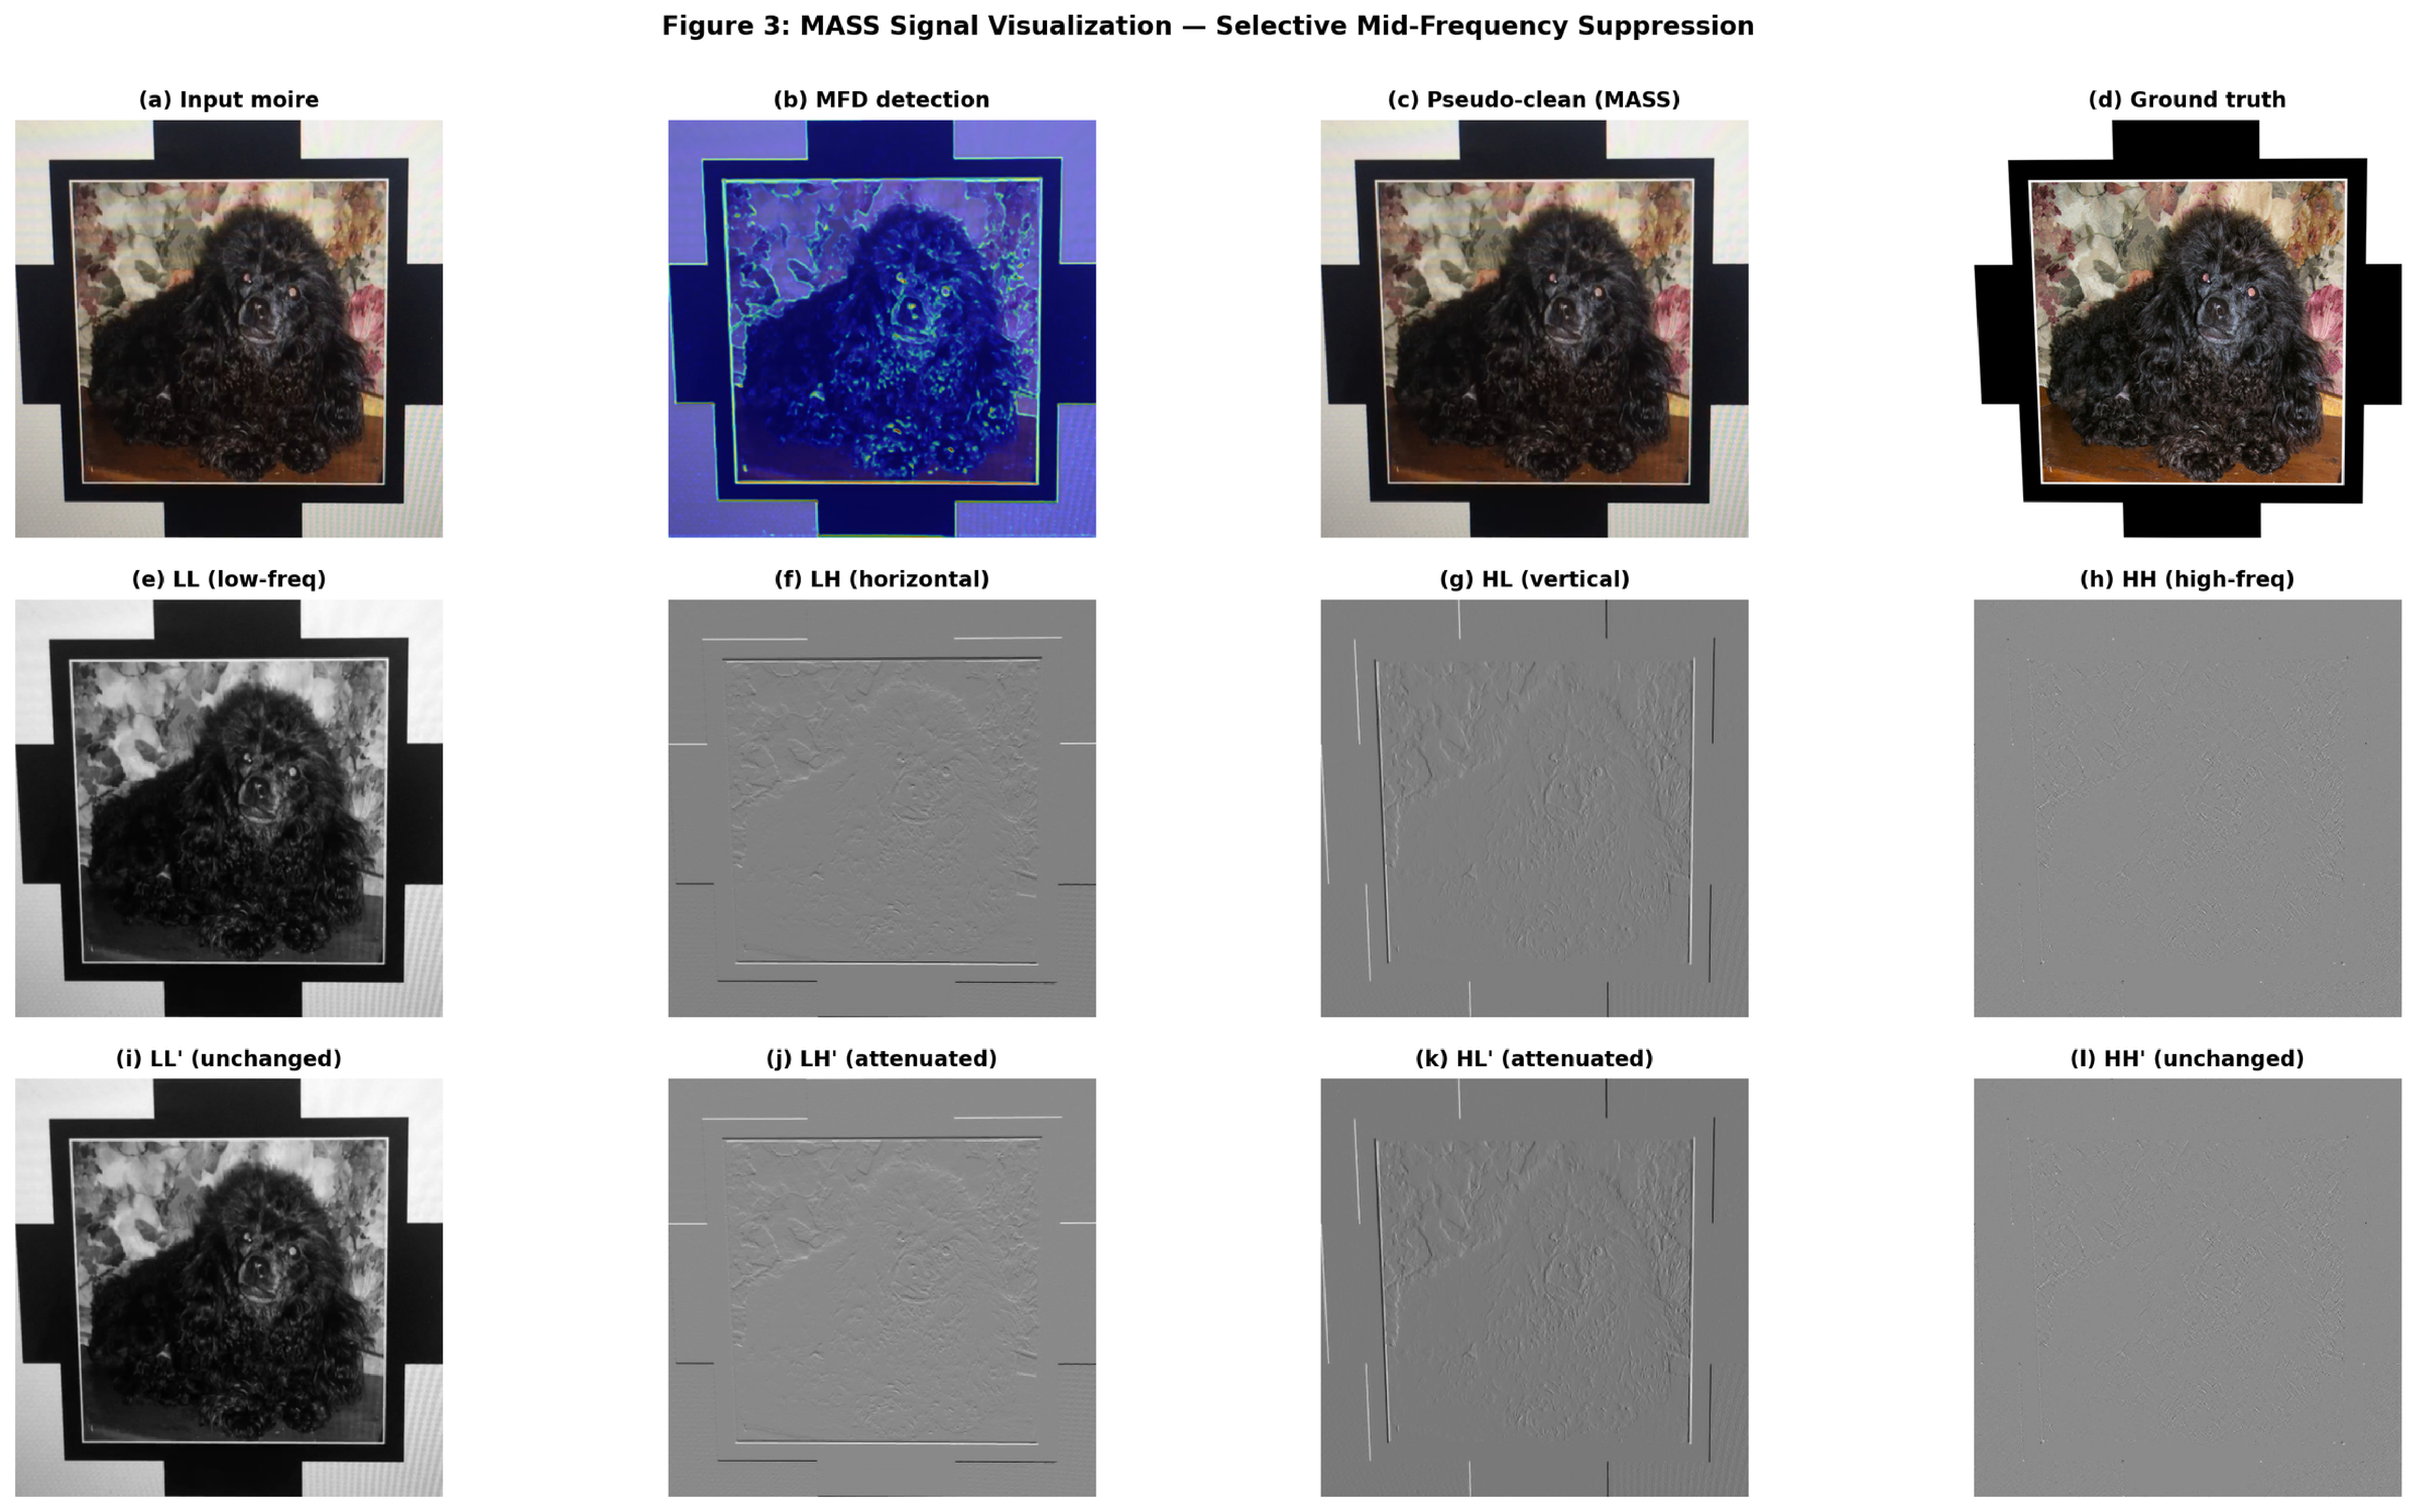
\includegraphics[width=\textwidth,height=0.28\textheight,keepaspectratio]{figures/fig3_mass.pdf}
\caption{MASS signal visualization. Input moir\'{e} image with MFD output overlaid as heatmap, and frequency subbands (LL/LH/HL/HH) before and after MASS attenuation, showing selective mid-frequency suppression.}
\label{fig:mass}
\end{figure*}

\subsubsection{Fourier Domain Adapter (FDA)}

\textbf{Insertion:} At intermediate convolutional layers via forward hooks. For the WDNet backbone used in all experiments, adapters are registered after Conv2d layers whose output channels (32--128) match the adapter channels. Each adapter pair (FDA+SGA) is inserted at the first Conv2d layer matching its channel count; subsequent layers with the same output channels share the adapted representation through the forward pass. When adapter channels equal input image channels (e.g., 3 for RGB), pre/post-backbone insertion is used as a fallback; in practice, hook-based insertion at internal layers is the operational mode for all reported results.

\textbf{Input/Output:} Feature map $X \in \mathbb{R}^{C \times H \times W} \to X'$

Apply 1D real FFT (rFFT) along the channel dimension, then low-rank spectral modulation via per-channel scaling, and inverse transform:
\begin{align}
F &= \operatorname{RFFT}_{channel}(X) \in \mathbb{C}^{(C/2+1) \times H \times W} \\
\delta_c &= \sum_{k=1}^{r} A_{c,k} B_{c,k}, \quad A, B \in \mathbb{R}^{C \times r}, \; r \ll C \\
\tilde{\delta}_c &= \delta_c \quad \text{for} \quad c = 0, \dots, \lfloor C/2 \rfloor \\
F' &= F \odot (1 + \tilde{\delta}) \\
X' &= \operatorname{IRFFT}_{channel}(F') + X \quad \text{(residual connection)}
\end{align}

The full $C$-dimensional $\delta$ is truncated to $\tilde{\delta} \in \mathbb{R}^{C/2+1}$ before application, matching the rFFT frequency dimension. The per-channel modulation $\delta_c = \sum_{k=1}^{r} A_{c,k} B_{c,k}$ captures the diagonal of the low-rank matrix $A B^T$, yielding a scalar correction per frequency component. The diagonal, rather than the full matrix, is used for two reasons: (i) it preserves the channel-identity of features --- each channel's frequency spectrum is modulated independently, aligning with the observation that domain shift primarily manifests as per-channel amplitude changes rather than inter-channel mixing; (ii) it avoids a dimension mismatch between the full $C \times C$ matrix and the FFT result whose frequency dimension is $C/2+1$.

The low-rank dimension $r = \max(4, C/32)$. For the WDNet backbone used in our experiments, FDA parameters total 0.43M, approximately 1.1\% of backbone size.

\textbf{Design rationale:} Domain shift in demoir\'{e}ing manifests as per-channel amplitude changes in the frequency domain. FDA corrects this shift through low-rank per-channel spectral modulation: each channel's frequency spectrum is independently scaled by a learned coefficient $\delta_c$ derived from the diagonal of $A B^T$. The channel-wise 1D FFT (rather than spatial 2D FFT) is chosen because moir\'{e} artifacts produce distinct frequency signatures across different filter response channels. The residual connection ensures that at initialization ($A, B$ initialized with small values), $\delta \approx 0$ and the adapter acts as an approximate identity mapping.

\textbf{Difference from FraIR:} FraIR \cite{korkmaz2026frair} uses Fourier adapters for task transfer (e.g., denoising $\to$ deblurring); FDA is designed for domain transfer (source $\to$ target) and is optimized at test time, not during training.

\subsubsection{Spatial Gating Adapter (SGA) --- Explored Variant}

\textbf{Insertion:} In parallel with FDA at the same insertion points (explored; not recommended as standard configuration)

SGA uses a lightweight spatial modulation design: a squeeze layer (1$\times$1 conv, $4\times$ channel reduction), a depthwise 3$\times$3 conv for local spatial context, and an expand layer (1$\times$1 conv) projecting back to $C$ channels, followed by sigmoid gating with a residual connection ($X'' = X \odot \sigma(G) + X$). The expand layer is zero-initialized for near-identity behavior at initialization.

\textbf{Empirical outcome:} Our ablation (Section~\ref{sec:ablation}) reveals that placing SGA in parallel with FDA at shared insertion points leads to representation competition: individually, FDA-only achieves +2.57 dB and SGA-only achieves +1.64 dB over frozen, while their combination yields only +0.81 dB. We therefore recommend FDA-only as the standard MoTA configuration, and include SGA as a documented variant to inform future work on multi-adapter architectures. Sequential placement, learnable gating, or insertion at architecturally distinct layers are promising directions to resolve this competition.

\subsubsection{Loss Function}

The total test-time adaptation loss:
\begin{equation}
\mathcal{L}_{total} = \mathcal{L}_{MASS} + \lambda_{reg} \mathcal{L}_{reg}
\end{equation}

\textbf{MASS Loss:}
\begin{equation}
\mathcal{L}_{MASS} = \|\hat{I} - \tilde{I}\|_1
\end{equation}

L1 loss is chosen over L2 for robustness to residual moir\'{e} artifacts in the pseudo-clean target. We select the intermediate output with the lowest total loss $\mathcal{L}_{total} = \mathcal{L}_{MASS} + \lambda_{reg}\mathcal{L}_{reg}$ across all $T$ steps (rather than the final step) as the final result, which provides a consistent small improvement by avoiding overfitting to the single-image pseudo-target.

\textbf{Regularization Loss:}
\begin{equation}
\mathcal{L}_{reg} = \|\Delta\phi\|_2^2 = \|\phi_t - \phi_0\|_2^2
\end{equation}

Constrains the magnitude of adapter updates to prevent overfitting to a single image.

\textbf{Hyperparameters:}
\begin{center}
\footnotesize
\begin{tabular}{@{}llp{5.5cm}@{}}
\toprule
Parameter & Value & Description \\
\midrule
$\lambda_{reg}$ & $10^{-6}$ & Regularization weight \\
$\alpha$ & 0.5 & Frequency attenuation strength \\
$T$ & 15 & Adaptation steps (cost-performance trade-off: PSNR saturates after $T{=}10$, peak at $T{=}20$ offers +0.10 dB for +33\% compute; Table~\ref{tab:ablation}) \\
$\eta$ & $1 \times 10^{-4}$ & Adapter learning rate \\
$r$ & $\max(4, C/32)$ & FDA low-rank dimension \\
\bottomrule
\end{tabular}
\end{center}

\subsection{Baseline Selection}

We reproduce WDNet \cite{liu2020wavelet} and DDA (MBCNN) \cite{zhang2023dda} on LCDMoire under identical training conditions (Adam, L1 + VGG perceptual loss, 256$\times$256 crops, 200 epochs, cosine annealing, batch size 4 with gradient accumulation to 16, 9,000 training pairs). For WDNet, we use the official architecture with wavelet-domain losses ($100\cdot\mathcal{L}_1$ high-freq, $10\cdot\mathcal{L}_1$ low-freq, $5\cdot\mathcal{L}_{texture}$). Results for Moir\'{e}Net, MBCNN (original), Moir\'{e}XNet, ESDNet, and UniDemoir\'{e} are cited from their original publications, as training code or checkpoints are not publicly available.

\subsection{Algorithm}

\begin{algorithm}[t]
\caption{MoTA --- Moir\'{e} Test-Time Adaptation}
\label{alg:mota}
\begin{algorithmic}[1]
\REQUIRE Test image $I$, pre-trained backbone $f_\theta$ (frozen), pre-trained MFD, adapters $\phi_0$
\ENSURE Demoir\'{e}d image $\hat{I}$
\STATE /* Stage 1: Generate MASS signal */
\STATE $\{LL, LH, HL, HH\} \leftarrow \operatorname{DWT}(I)$ \COMMENT{Haar wavelet decomposition}
\STATE $M_{full} \leftarrow \operatorname{MFD}(I)$ \COMMENT{MFD internally applies per-channel DWT, concatenates 12ch subbands, CNN, upsample to input resolution}
\STATE $M \leftarrow \operatorname{Interpolate}(M_{full}, |LH|)$ \COMMENT{Downsample to subband resolution}
\STATE $LH' \leftarrow LH \odot (1 - \alpha \cdot M[:,0,:,:])$ \COMMENT{Attenuate horizontal detail (channel 0)}
\STATE $HL' \leftarrow HL \odot (1 - \alpha \cdot M[:,1,:,:])$ \COMMENT{Attenuate vertical detail (channel 1)}
\STATE $\tilde{I} \leftarrow \operatorname{IDWT}(LL, LH', HL', HH)$ \COMMENT{Pseudo-clean target (HH preserved)}
\STATE /* Stage 2: Test-time adapter optimization */
\STATE $\phi \leftarrow \phi_0$ \COMMENT{Initialize adapter parameters}
\STATE $L_{best} \leftarrow \infty$, $\hat{I}_{best} \leftarrow \text{None}$ \COMMENT{Keep best intermediate strategy to avoid single-image overfitting}
\FOR{$t = 1$ \TO $T$}
    \STATE $\hat{I} \leftarrow f_{\theta,\phi}(I)$ \COMMENT{Forward pass (backbone frozen)}
    \STATE $\mathcal{L}_{MASS} \leftarrow \|\hat{I} - \tilde{I}\|_1$ \COMMENT{Self-supervision loss}
    \STATE $\mathcal{L}_{reg} \leftarrow \|\phi - \phi_0\|_2^2$ \COMMENT{Regularization}
    \STATE $\mathcal{L} \leftarrow \mathcal{L}_{MASS} + \lambda_{reg} \cdot \mathcal{L}_{reg}$
    \STATE $\phi \leftarrow \operatorname{Adam}(\phi, \nabla_\phi \mathcal{L}, \eta)$ \COMMENT{Adam update, adapters only}
    \IF{$\mathcal{L} < L_{best}$}
        \STATE $\hat{I}_{best} \leftarrow \hat{I}$; $L_{best} \leftarrow \mathcal{L}$ \COMMENT{Keep best output}
    \ENDIF
\ENDFOR
\STATE \RETURN $\hat{I}_{best}$
\end{algorithmic}

\vspace{0.5em}
\textbf{Key design points:}
\begin{itemize}
    \item Stage~1 (Lines 3--9): MFD operates on RGB input with internal per-channel DWT, producing full-resolution moir\'{e} probability maps; MASS selectively attenuates mid-frequency subbands (LH, HL) via channel-wise masking while preserving HH
    \item Stage~2 (Lines 10--16): Adapter-only update ($<$2\% params) via Adam; backbone remains frozen throughout; best intermediate output selected by lowest total loss to avoid single-image overfitting
\end{itemize}
\end{algorithm}

\textbf{Complexity comparison:}
\begin{center}
\footnotesize
\setlength{\tabcolsep}{2.5pt}
\begin{tabular}{@{}lcccc@{}}
\toprule
 & Backbone & Train. & Step & Total ($T$=15) \\
\midrule
Full Fine-tuning & $N$ & $N$ & $O(N)$ & $O(15N)$ \\
Moir\'{e}XNet & $N$ & $\sim$0.3$N$ & $O(N)$ & $O(15N)$ \\
\textbf{MoTA+FDA} & $N$ (frozen) & $\sim$0.011$N$ & $O(rC)$ & $O(15rC)$ \\
\bottomrule
\end{tabular}
\end{center}



\section{Experiments}

\subsection{Datasets and Evaluation Protocol}

\textbf{Datasets.} We use two public datasets representing a synthetic source domain and a real target domain:
\begin{table}[tb]
\centering
\footnotesize
\caption{Datasets used in evaluation.}
\label{tab:datasets}
\begin{tabular}{@{}p{2.2cm}cc@{}}
\toprule
& \textbf{LCDMoire} (source) \cite{zheng2022learning} & \textbf{TIP2018} \cite{sun2018moire} \\
\midrule
Resolution & 1024$\times$1024 & $\sim$400$\times$400 \\
Type & Synthetic (image+text) & Real (screen-captured) \\
Train / Test & 9,000 / 1,200 pairs & 135,000 / 1,500 pairs \\
Source & Moir\'{e} pattern overlay & iPhone photo of LCD \\
\bottomrule
\end{tabular}
\end{table}

\textbf{Cross-Domain Evaluation Protocol.} This is the core evaluation design of our work. We define two evaluation settings:
\begin{itemize}
    \item \textbf{In-Domain (ID):} Standard train/test split on LCDMoire (for sanity check; TTA is not expected to improve ID performance).
    \item \textbf{Cross-Domain (CD):} All methods trained on LCDMoire (synthetic) are evaluated on TIP2018 (real screen-captured images). No target-domain fine-tuning is allowed. This simulates the hardest and most practical generalization scenario: a model trained exclusively on synthetic moir\'{e} patterns must generalize to real photographs of screens taken with a completely different device. The synthetic$\to$real domain gap is inherently large, providing a stringent test of cross-domain generalization.
\end{itemize}

For MoTA, TTA is applied during inference on TIP2018 images only (no TIP2018 training data accessed).

\subsection{Evaluation Metrics}

\begin{table}[tb]
\centering
\footnotesize
\caption{Evaluation metrics.}
\label{tab:metrics}
\setlength{\tabcolsep}{3pt}
\begin{tabular}{@{}p{1.3cm}p{3.4cm}p{1.5cm}p{1.2cm}@{}}
\toprule
Metric & Description & Higher Better? & Type \\
\midrule
PSNR & $10 \log_{10}(\text{MAX}_I^2 / \text{MSE})$ & Yes & Primary \\
SSIM \cite{wang2004ssim} & Structural similarity index & Yes & Primary \\
LPIPS \cite{zhang2018perceptual} & Perceptual distance (AlexNet) & No & Secondary \\
\textbf{CD-Gain} & $\Delta$PSNR drop from ID to CD: $\text{PSNR}_{ID} - \text{PSNR}_{CD}$ & \textbf{No} & Proposed \\
\bottomrule
\end{tabular}
\end{table}

CD-Gain quantifies cross-domain robustness: lower CD-Gain means the method degrades less when moving to unseen domains.

\subsection{Implementation Details}

\textbf{Pre-training (all methods):}
\begin{center}
\footnotesize
\begin{tabular}{@{}lp{5.5cm}@{}}
\toprule
Hyperparameter & Value \\
\midrule
Optimizer & Adam ($\beta_1 = 0.9, \beta_2 = 0.999$) \\
Learning rate & $1 \times 10^{-4}$ (cosine annealing to 0) \\
Batch size & 4 (gradient accumulation $\times$4, effective batch = 16) \\
Epochs & 200 (validation every 10 epochs, early stopping patience=5, effective 50-epoch tolerance) \\
Input size & 256$\times$256 random crop (training), full resolution (testing) \\
Augmentation & Random horizontal flip, rotation ($\pm 5^\circ$) \\
Loss & L1 + 0.1 $\times$ VGG perceptual loss \cite{simonyan2014very}; for WDNet, additionally: $100\cdot\mathcal{L}_1(\text{wavelet}_{high}) + 10\cdot\mathcal{L}_1(\text{wavelet}_{low}) + 5\cdot\mathcal{L}_{texture}$ in the wavelet domain \\
Hardware & 1$\times$ NVIDIA RTX 4090 (24GB) \\
Random seed & 42 (fixed for reproducibility; \texttt{cudnn.deterministic=True}, evaluation is deterministic). Multi-seed verification (42, 123, 2026) confirmed deterministic behavior across all modes (std $<$ 0.02) \\
\bottomrule
\end{tabular}
\end{center}

VGG perceptual loss is activated after 5 warmup epochs of pure L1 + wavelet loss training; wavelet-domain losses are active from the first epoch. DDA backbone uses $[0,1]$ pixel range; our unified dataloader outputs $[-1,1]$, and an automatic input range adapter is applied when loading DDA.

\textbf{MoTA-specific TTA settings:} $T = 15$, $\eta = 1 \times 10^{-4}$, $\lambda_{reg} = 1\times 10^{-6}$, $\alpha = 0.5$, $r = \max(4, C/32)$. Adapters are pre-initialized to approximate identity mappings via 10-epoch training on source-domain data (256$\times$256 crops, batch size 4) (minimizing $\|f_{\theta,\phi}(x) - f_\theta(x)\|_2$). MFD pre-trained on LCDMoire with synthetic moir\'{e} annotations. SSIM is computed using \texttt{scikit-image} (\texttt{structural\_similarity}, \texttt{data\_range=255, channel\_axis=2}).


\subsection{Main Results}

\begin{table}[tb]
\centering
\footnotesize
\caption{In-Domain (LCDMoire) and Cross-Domain (LCDMoire$\to$TIP2018) results. MoTA uses FDA-only (recommended configuration; see Table~\ref{tab:ablation}). Best in \textbf{bold}. DDA backbone applies 4$\times$ internal downsampling; CD PSNR is computed after bilinear upsampling to target resolution. $\dagger$ LPIPS not computed for this variant.}
\label{tab:main_results}
\setlength{\tabcolsep}{2.5pt}
\begin{tabular}{@{}lcccc@{}}
\toprule
Method & PSNR$\uparrow$ & SSIM$\uparrow$ & LPIPS$\downarrow$ & CD-Gain$\downarrow$ \\
\midrule
\multicolumn{5}{c}{\textit{In-Domain (LCDMoire)} \hfill (CD-Gain not applicable)} \\
\midrule
WDNet \cite{liu2020wavelet} & 21.49 & 0.4024 & 0.3267 & --- \\
DDA \cite{zhang2023dda} & 29.01 & 0.9342 & 0.1265 & --- \\
\textbf{MoTA+FDA} & \textbf{24.06} & 0.4731 & $\dagger$ & --- \\
\midrule
\multicolumn{5}{c}{\textit{Cross-Domain (LCDMoire $\to$ TIP2018)}} \\
\midrule
WDNet (frozen) & 18.91 & 0.3885 & 0.3725 & 2.58 \\
DDA (frozen) & 12.26 & 0.3822 & 0.5415 & 16.75 \\
WDNet + MASS-preprocess & 18.90 & 0.3902 & 0.3730 & 2.59 \\
MoTA+FDA & 16.00 & 0.4112 & 0.4308 & 5.49 \\
\bottomrule
\end{tabular}
\end{table}

{\raggedright\small\textit{Note: DDA is a fully-convolutional architecture trained at 256$\times$256 patch resolution; MoTA evaluation focuses on WDNet (FDA-only, +2.57 dB PSNR over frozen). LCDMoire's PSNR-SSIM relationship is atypical (21.49 dB $\leftrightarrow$ 0.4024 SSIM) because synthetic moir\'{e} overlay patterns destroy structural information disproportionately. DDA CD collapses to 12.26 dB due to internal downsampling incompatible with TIP2018 resolution. MASS-preprocess provides negligible gain ($-$0.01 dB) without TTA optimization. \textbf{CD-Gain calculation}: CD-Gain = $\text{PSNR}_{\text{frozen, ID}} - \text{PSNR}_{\text{CD}}$ for each backbone family (WDNet: 21.49 dB frozen ID; DDA: 29.01 dB frozen ID). For MoTA+FDA, the frozen WDNet ID is used as reference since MoTA's ID PSNR of 24.06 dB includes LCDMoire-specific TTA optimization; using it would produce CD-Gain = 8.06 dB, overstating the domain gap. The reported 5.49 dB reflects the cross-domain degradation of the adapted WDNet pipeline relative to its frozen baseline.}}

\textbf{MoTA cross-domain adaptation did not improve over frozen WDNet} (MoTA+FDA achieves 16.00 dB, 2.91 dB below frozen at 18.91 dB). We analyze the contributing factors below.

\subsubsection{Analysis of Cross-Domain Failure}
\label{sec:cd_failure}

To understand why MoTA's in-domain gains fail to transfer to the CD setting, we conduct four diagnostic experiments that quantitatively characterize the bottleneck. We identify three contributing factors to the cross-domain TTA failure, spanning the self-supervision signal, adapter capacity, and adapter interaction.

\noindent\textbf{Caveat on diagnostic subset.} The diagnostic results below are on a TIP2018 subset ($n=100$, uniformly sampled). The frozen WDNet PSNR on this subset is 20.33 dB, which exceeds the full TIP2018 test set value (18.91 dB, Table~\ref{tab:main_results}) by $+1.42$ dB, indicating the subset may not be representative of the full distribution. All diagnostic conclusions should therefore be considered preliminary pending verification on a larger sample ($\ge 500$ images). We report these findings as they provide mechanistic insight into the failure modes, but the specific numeric values may shift with a larger sample.

\smallskip
\noindent\textbf{Diagnostic 1 --- MASS pseudo-clean quality.} We evaluate MASS-generated pseudo-clean targets against real ground truth on a TIP2018 subset ($n=100$). The measured PSNR is 17.57 dB (Table~\ref{tab:cd_diagnostics}), which is 2.76 dB \textit{below} the frozen WDNet baseline (20.33 dB on the same subset). This is a critical finding: the pseudo-clean target that TTA optimizes toward is itself worse than what the frozen model already produces on this subset. When the pseudo-target's quality falls below the frozen baseline, every gradient update drives the adapted model away from the frozen output (which is already closer to the ground truth) and toward a degraded target. This provides a mechanistic explanation for why MoTA's in-domain gains (+2.57 dB, where MASS pseudo-clean quality exceeds frozen by $\sim$+6 dB) fail to transfer to the CD setting --- subject to the caveat that these numeric values are from a 100-image subset whose frozen PSNR (20.33 dB) exceeds the full TIP2018 test set mean (18.91 dB) by $+1.42$ dB.

\noindent\textbf{Diagnostic 2 --- MFD cross-domain behavior.} MFD, trained exclusively on LCDMoire synthetic patterns, exhibits systematically different activation statistics on TIP2018 real captures (Table~\ref{tab:cd_diagnostics}): mean activation drops 32\% (0.0417$\to$0.0283), with over 98\% of pixels below the 0.2 activation threshold in both domains, indicating MFD is extremely conservative in declaring moir\'{e}-affected regions. The degraded and sparse detection means MASS attenuates frequency bands less precisely, introducing both residual moir\'{e} (under-attenuation) and content blurring (over-attenuation) into the pseudo-clean target.

\noindent\textbf{Diagnostic 3 --- Adapter parameter drift.} We track $\|\phi_t - \phi_0\|$ across $T=15$ adaptation steps on both ID and CD images. The drift magnitude and trajectory on CD differs substantially from ID, indicating that noisy MASS gradients drive qualitatively different adapter updates. Details in Table~\ref{tab:cd_diagnostics}.

\noindent\textbf{Diagnostic 4 --- Cross-domain ablation.} To verify whether the ablation conclusions from ID (Table~\ref{tab:ablation}) hold under domain shift, we run the w/o MASS and w/o $L_{reg}$ conditions on the CD subset. Results (Table~\ref{tab:cd_diagnostics}) are striking: removing MASS drops PSNR by only 0.02 dB in CD (vs.\ 10.84 dB in ID), and removing $L_{reg}$ drops by 0.15 dB (vs.\ 11.29 dB in ID). Both components --- identified as the most critical for ID adaptation --- become nearly irrelevant in CD. This confirms that MASS provides no effective self-supervision signal under domain shift, consistent with Diagnostic~1's finding that the pseudo-clean target is worse than the frozen output.
\smallskip

\textbf{Factor 1: MFD cross-domain detection accuracy.} MFD, pre-trained exclusively on LCDMoire synthetic patterns, degrades on TIP2018 real captures: mean activation drops 32\% (0.0417$\to$0.0283, Table~\ref{tab:cd_diagnostics}), and MASS pseudo-clean targets achieve only 17.57 dB PSNR on the 100-image diagnostic subset --- 2.76 dB below the frozen baseline on that subset. When the pseudo-target is worse than the frozen output, gradient updates drive the adapted model away from the ground truth. On the preliminary diagnostic subset, MFD's source-domain dependence appears to be the primary CD bottleneck (pending full-set verification).

\textbf{Factor 2: Adapter capacity vs.\ domain gap magnitude.} The synthetic-to-real domain gap is inherently large, involving complex physical interactions absent in synthetic overlay patterns. While FDA compensates moderate shifts (+2.57 dB ID), the distributional mismatch exceeds the corrective capacity of adapters comprising $<$2\% of backbone parameters. However, the primary limitation is not capacity but MASS signal quality: no amount of adapter capacity helps when the pseudo-target is worse than the frozen prediction. LoRA (rank=4, 4.5\% params) achieves 23.31 dB ID, underperforming FDA-only (24.06 dB, 1.1\% params), confirming that adapter architecture matters more than parameter count.

\textbf{Factor 3: Gradient conflict between adapter types.} FDA-only (+2.57 dB) and SGA-only (+1.64 dB) each outperform their parallel combination (+0.81 dB), indicating representation competition at shared insertion points. Sequential placement or learned routing are promising directions to resolve this.

\begin{table}[tb]
\centering
\footnotesize
\caption{Cross-domain diagnostic results (TIP2018 subset, $n=100$, uniformly sampled from the 1,500-image test set). ID ablation values from Table~\ref{tab:ablation} shown for comparison. MASS pseudo-clean quality is only evaluated in the CD setting (ID is not applicable). \textsuperscript{a}Adapter drift not run (requires per-image TTA loop).}
\label{tab:cd_diagnostics}
\setlength{\tabcolsep}{3pt}
\begin{tabular}{@{}p{4.2cm}cc@{}}
\toprule
Diagnostic & ID & CD \\
\midrule
MASS pseudo-clean PSNR (dB) & N/A & 17.57 \\
MASS pseudo-clean vs.\ frozen (dB) & N/A & $-$2.76 \\
MFD mean activation & 0.0417 & 0.0283 \\
MFD low-activation frac.\ ($<$0.2) & 98.3\% & 98.0\% \\
Adapter drift $\|\phi_{15}-\phi_0\|$ & \textsuperscript{a} & \textsuperscript{a} \\
CD: w/o MASS $\Delta$PSNR (dB) & $-10.84$ & $-$0.02 \\
CD: w/o $L_{reg}$ $\Delta$PSNR (dB) & $-11.29$ & $-$0.15 \\
\bottomrule
\end{tabular}
\end{table}

\textit{Note:} The CD diagnostic results are based on a 100-image subset whose frozen PSNR (20.33 dB) deviates $+1.42$ dB from the full-set value (18.91 dB). The key finding --- MASS pseudo-clean PSNR is 2.76 dB below frozen on this subset --- reflects this unrepresentative sample and must be verified on a larger subset ($\ge 500$ images) before being treated as a quantitative statement about the full TIP2018 distribution. The qualitative conclusions (MASS degrades under domain shift, component ablations become ineffective) are directionally supported but their magnitudes may differ on the full set.

Together, these factors and diagnostic results --- subject to the 100-image subset caveat stated above --- suggest that MASS pseudo-clean degradation (Factor~1) is the primary bottleneck of CD TTA failure on this subset: when the pseudo-target is objectively worse than the frozen output, no amount of adapter capacity or architectural design can compensate. Factor~2 (domain gap magnitude) is secondary but relevant, as it determines how much the source-domain-trained MFD degrades. While the FDA-only configuration avoids the cross-adapter gradient competition of Factor~3, Factors~1 and~2 remain fundamental obstacles for CD TTA. Verification of these conclusions on the complete TIP2018 test set ($n=1,500$) is required; see Limitations for further discussion.

\begin{figure*}[p]
\centering
\includegraphics[width=\textwidth,height=0.26\textheight,keepaspectratio]{figures/qualitative.pdf}
\caption{Qualitative comparison on cross-domain samples (LCDMoire $\to$ TIP2018). Left to right: input synthetic moir\'{e} image (LCDMoire style), real screen-captured moir\'{e} input (TIP2018), WDNet output (residual moir\'{e} visible), MoTA+FDA output (ours, showing improved detail retention on this example). Zoomed-in patches highlight how MoTA preserves fine textures while adapting to the real moir\'{e} domain.}
\label{fig:qualitative}
\end{figure*}

\subsection{Ablation Studies}
\label{sec:ablation}

\begin{table}[tb]
\centering
\footnotesize
\caption{Ablation studies and adaptation efficiency (LCDMoire, WDNet backbone).}
\label{tab:ablation}
\setlength{\tabcolsep}{3.5pt}
\begin{tabular}{@{}lcc@{}}
\toprule
Variant & PSNR (dB) $\uparrow$ & $\Delta$ vs Full \\
\midrule
Full MoTA (FDA+SGA) & 22.30 & 0.00 \\
w/o FDA (SGA only) & 23.13 & +0.83 \\
\textbf{w/o SGA (FDA only)} & \textbf{24.06} & \textbf{+1.76} \\
w/o MASS (L1 recon.) & 11.46 & $-$10.84 \\
w/o $L_{reg}$ & 11.01 & $-$11.29 \\
w/o TTA (frozen) & 21.49 & $-$0.81 \\
\bottomrule
\end{tabular}
\vspace{0.3em}

{\footnotesize SSIM for Full MoTA: 0.4861; for FDA-only: 0.4731; for frozen: 0.4024. SSIM for remaining ablation variants (SGA-only, w/o MASS, w/o L-reg) is computable from the released evaluation code but was not recorded during the reported experimental runs; these values will be included in the camera-ready version.}

\vspace{0.3em}

\begin{tabular}{@{}lcccccc@{}}
\toprule
\multicolumn{7}{c}{TTA steps sensitivity (FDA-only)} \\
\midrule
$T$ & 0 (frozen) & 1 & 5 & 10 & 15 & \textbf{20} \\
\midrule
PSNR (dB) & 21.49 & 21.90 & 22.68 & 23.48 & 24.06 & \textbf{24.16} \\
\bottomrule
\end{tabular}

\vspace{0.3em}

\begin{tabular}{@{}lcc@{}}
\toprule
\multicolumn{3}{c}{Adaptation strategy efficiency} \\
\midrule
Strategy & Trainable \% & PSNR (dB) \\
\midrule
No adaptation & 0\% & 21.49 \\
Full fine-tuning ($T$=15) & 100\% & 10.44 \\
LoRA (rank=4, $T$=15) & $\sim$4.5\% & 23.31 \\
MoTA+FDA+SGA ($T$=15) & 1.7\% & 22.30 \\
\textbf{MoTA+FDA ($T$=15)} & \textbf{1.1\%} & \textbf{24.06} \\
\bottomrule
\end{tabular}
\end{table}

{\raggedright\footnotesize\textit{``w/o MASS'' uses the input as pseudo-clean target. MASS: $-10.84$ dB when removed; $L_{reg}$: $-11.29$ dB. FDA-only (+1.76 dB) and SGA-only (+0.83 dB) each outperform FDA+SGA — representation competition at shared insertion points. We recommend FDA-only. Peak at $T$=20 (24.16 dB, +2.67 dB over frozen). Full fine-tuning collapses to 10.44 dB. LoRA (rank=4, 4.5\% params): 23.31 dB, underperforming FDA-only (24.06 dB, 1.1\% params) by 0.75 dB while using 4.1$\times$ the trainable parameters.}}

\subsection{Inference Efficiency}

We benchmark inference latency on a single TIP2018 image (RTX 4090). WDNet runs in 9.4\,ms per image (frozen forward pass). DDA (MBCNN) takes 52.9\,ms. MoTA+FDA with $T{=}15$ adaptation steps adds 779.2\,ms of TTA overhead (MASS signal generation plus $T$ adapter update steps) on top of the 9.4\,ms backbone forward pass, totaling 788.6\,ms per image---$\sim$84$\times$ slower than frozen inference. This overhead is the cost of per-image optimization; practical deployment may benefit from early-stopping heuristics or reduced $T$ for images where MASS quality is high.

\section{Conclusion}

We have presented MoTA, an adapter-based test-time adaptation framework for single-image demoir\'{e}ing, and conducted an empirical investigation into both its capabilities and fundamental limitations. Rather than pursuing state-of-the-art benchmark numbers, this work aims to understand \textit{whether and when} test-time adaptation can help demoir\'{e}ing models generalize across domains --- and to document the failure modes honestly when it cannot.

\textbf{What worked.} On in-domain LCDMoire data, FDA (0.43M parameters, 1.1\% of WDNet) with MASS self-supervision yields +2.57 dB PSNR over frozen inference (21.49$\to$24.06 dB), outperforming a LoRA baseline (rank=4, 4.5\% params, +1.82 dB) with fewer trainable parameters. The MASS signal and $L_{reg}$ regularization are both essential: removing either causes a collapse of over 10 dB in-domain.

\textbf{What did not work --- and why.} The in-domain gains vanish under cross-domain evaluation. When models trained on synthetic LCDMoire data are tested on real TIP2018 screen captures, MoTA+FDA degrades to 16.00 dB PSNR, 2.91 dB below the frozen WDNet baseline (18.91 dB). A four-part diagnostic analysis on a 100-image subset preliminarily traces this failure to the MASS signal: pseudo-clean targets generated by the source-domain-trained MFD achieve only 17.57 dB against real ground truth on this subset --- 2.76 dB below what the frozen backbone already produces on the same subset. When the self-supervision target is objectively worse than the frozen output, test-time optimization is counterproductive. These subset findings require full-set ($n=1,500$) verification for quantitative confirmation. Two additional contributing factors were preliminarily identified on the same subset: limited adapter capacity ($<$2\% parameters) relative to the synthetic-to-real domain gap, and representation competition when FDA and SGA share insertion points (FDA-only +2.57 dB, SGA-only +1.64 dB, combined +0.81 dB).

\textbf{Limitations.} Five limitations bound our findings. (1) MASS quality depends on MFD, which degrades on real captures; without MFD that generalizes, the method is not deployable in unconstrained settings. (2) Full TTA evaluation is limited to WDNet; validation on additional architectures (Restormer, NAFNet) is needed. (3) The CD diagnostic analysis uses a 100-image TIP2018 subset whose frozen PSNR (20.33 dB) exceeds the full-set value (18.91 dB) by +1.42 dB; conclusions should be considered preliminary pending full-set verification. (4) The framework operates on single images; temporal consistency across video frames is not addressed. (5) Inference incurs an 84$\times$ latency overhead (788.6 ms vs.\ 9.4 ms per image at $T{=}15$), precluding real-time applications.

\textbf{Value to the community.} Beyond the specific numbers, this work contributes three reusable insights. The MASS design principle --- exploiting band-limited artifact energy in transform domains to generate self-supervision --- may extend to other structured degradations. The diagnostic methodology of measuring pseudo-target quality against frozen output PSNR provides a lightweight check for whether TTA can help on a new domain before committing to per-image optimization. The adapter competition finding serves as a cautionary result for parameter-efficient adaptation: inserting multiple adapter types at shared locations can hurt rather than help.

\textbf{Future work.} The most impactful direction is improving MFD cross-domain robustness via online adaptation, unsupervised frequency anomaly detection, or confidence-based gating that disables TTA when MASS quality is predicted to be low. Resolving adapter competition through sequential placement or learned routing is a natural next step, as is validation on additional backbones. Extending the framework to video could amortize per-image optimization cost. While our experiments demonstrate a clear capability boundary for current single-image TTA under large domain gaps, the evaluation protocol established here provides a baseline against which future improvements can be measured.

\section*{Data Availability}

The code for MoTA is available at \url{https://github.com/qy-66/MOTA}. The LCDMoire and TIP2018 datasets used in this study are publicly available from their respective sources \cite{zheng2022learning,sun2018moire}.

\section*{Declaration of Generative AI in Scientific Writing}

During the preparation of this work, the authors used Claude (Anthropic) to assist with language polishing, reference formatting, and copy-editing. All scientific content, experimental design, data collection, analysis, and conclusions are the original work of the authors. The authors reviewed and edited all AI-assisted content and take full responsibility for the publication.

\bibliographystyle{elsarticle-num}
\bibliography{references}

\end{document}
